\section{Introductie}

Aan de hand van de projectopdracht, ons Plan van Aanpak en gesprekken met Johan en Cor-Paul hebben we dit Orientatieverslag opgesteld. Dit verslag zal worden gebruikt om inzicht te verkrijgen in de mogelijke technieken voor het ontwikkelen van mobiele applicaties en server back-ends, geschikt voor onze toepassing. Tevens zullen we hier onze keuzes voor bepaalde technieken motiveren.

\section{Back-end}\label{sec:orientatie-back-end}
Afhankelijk van welk back-end platform we kiezen, zijn er verschillende mogelijkheden voor de servers waarop de back-end kan draaien. Ook is er de keuze tussen traditionele server clusters en een cloud-oplossing, zoals een \ac{paas}. Er zijn verschillende redenen om wel of niet voor een cloud oplossing te gaan. Deze voor- en nadelen hadden wij vooraf in gedachten: 
\begin{itemize} 
    \item[+] Automatisch en vrijwel onbeperkt schaalbaar
    \item[+] Opzetten besturingssysteem is niet nodig/kan niet
    \item[-] Mogelijk duurder vanwege winstmarge \ac{paas}
    \item[-] Minder keuze in hoeveelheid beschikbare talen/frameworks
\end{itemize}

Het nadeel dat de prijs hoger kan liggen kan worden afgezwakt en mogelijk worden omgebogen: om grote hoeveelheden gebruikers aan te kunnen moet een traditioneel server cluster groot zijn, terwijl een \ac{paas} automatisch kan schalen en dus op dal-momenten significant goedkoper kan zijn. We verwachten dat het gebruik van onze applicatie een piek zal vertonen in de avond en in het weekend, omdat er voornamelijk buiten werk en schooltijd gesport wordt. Er is voor onze applicatie dus meer dal- dan piek-belasting en we verwachten dus ook dat een \ac{paas} oplossing goedkoper zal zijn dan een cluster.

In tabel~\ref{tab:paas} ziet u een overzicht van de verschillende grote cloud platformen die er momenteel zijn, en de talen en frameworks die ze ondersteunen~\cite{paas-list-tomsitpro, azure-scala, aws}. Zoals in de tabel te zien is ondersteunen de meeste \acp{paas} een heleboel talen en frameworks. Microsoft Azure en Amazon AWS ondersteunen de 4 grote platformen .NET, Java, Python en NodeJS.

\begin{table}
\caption {Vijf grote \ac{paas} providers en de talen en frameworks die ze ondersteunen} \label{tab:paas} 
\begin{tabular}{lccccc}
\textbf{}        & \multicolumn{1}{l}{\textbf{Azure}} & \multicolumn{1}{l}{\textbf{GAE}} & \multicolumn{1}{l}{\textbf{AWS}} & \multicolumn{1}{l}{\textbf{Heroku}} & \multicolumn{1}{l}{\textbf{AppFog}} \\
\textbf{.NET}    & x &   & x &   &   \\
\textbf{Java}    & x & x & x & x & x \\
\textbf{Scala}   & x & x & x & x & x \\
\textbf{Python}  & x & x & x &   & x \\
\textbf{Node.JS} & x &   & x & x & x \\
\textbf{PHP}     & x & x & x &   & x \\
\textbf{Ruby}    & x &   & x & x & x \\
\textbf{Overig}  &   & Go & & Closure & Erlang
\end{tabular}
\end{table}

De bestaande systemen van Emando zijn gemaakt met het .NET framework en draaien voornamelijk in Microsoft Azure als Cloud Service. Aangezien MyLaps voor ons een belangrijke databron is en de MyLaps SDK alleen voor C\#/.NET beschikbaar is, kan er veel werk bespaard worden door ook deze programmeertaal en runtime te gebruiken. 

Bovendien heeft Emando een laag over de MyLaps SDK heen geschreven waardoor de SDK bruikbaar is met \acf{rx}. \ac{rx} - mede ontwikkeld door prof.dr. H.J.M. Meijer~\cite{meijer2011world} - is een manier om LINQ te gebruiken voor observeerbare collecties en asynchroon programmeren, twee eigenschappen waar we met onze applicatie mee te maken gaan krijgen.

We hebben ook de andere platformen overwogen, maar door gebrek aan de MyLaps SDK en het gebruik van .NET door Emando waren dit geen echte opties.

\subsection{Real-time}\label{sec:orientatie-real-time}
De trainingsapplicatie moet zonder dat de gebruiker de applicatie handmatig ververst de laatste doorkomsten binnenkrijgen en tonen. Ook moet de getoonde rondetijd up to date zijn, en niet een ronde tijd van een vorig rondje. De communicatie tussen de back-end en de clients moet dus real-time zijn. Real-time wil zeggen dat de server een update naar de client kan sturen. In `normaal' web verkeer kan de server niet op elk moment een bericht sturen naar de client. De server kan alleen reageren op een verzoek van de client, omdat de client geen vast IP-adres heeft en er standaard geen poort open staat. Pas wanneer de client een uitgaand verzoek heeft gaat er een poort open.

Een oplossing hiervoor is WebSockets: bij WebSockets blijft de verbinding open en dus de poort en kan de server op elk moment een bericht sturen, als er bijvoorbeeld een schaatser voorbij een detectie-lus komt. Een verbinding openhouden kost wel geheugen op de server en de server heeft dus een maximum aantal verbindingen dat hij kan openhouden. Er bestaan verschillende WebSocket frameworks die je het aanmaken en onderhouden van de verbindingen uit handen nemen. Een hiervan is SignalR voor .NET. Emando heeft SignalR succesvol gebruikt tijdens de Olympische Spelen van 2014 om \url{http://live.schaatsen.nl} te voorzien van live data. SignalR is inmiddels een officiele ASP.NET library\footnote{http://www.asp.net/signalr} en wordt ontwikkeld en ondersteund door Microsoft ontwikkelaars.

\section{Client}
Er zijn tegenwoordig diverse manieren om mobiele applicaties te maken, voor diverse platformen (iOS, Android, Windows Phone). Deze verschillende methodes vereisen verschillende programmeertalen en architecturen. Een groot verschil tussen de verschillende methodes is de hoeveelheid code die kan worden hergebruikt tussen verschillende platformen. De uiterste daarvan zijn gebruiken een compleet gescheiden broncode versus een volledig gedeelde broncode. De volgende methodes hebben we overwogen:

\begin{description}
\item[Native applicatie:] Een native applicatie is een applicatie die ontworpen is voor een specifiek platform. Het design van dergelijke applicaties ligt (meestal) in het verlengde van de richtlijnen voor dit platform en het gebruik van platform specifieke handelingen (gestures) wordt gestimuleerd en gehanteerd binnen de applicatie. Vanwege de richtlijnen en het gebruik van deze gestures, zijn dergelijke applicaties zelfverklarend voor eindgebruikers. Een ander voordeel is dat door de native implementatie, de user interface performance van dergelijke applicaties doorgaans erg goed is.

Een nadeel van native applicaties is dat applicatie code vaak in een platform specifieke programmeertaal wordt ontwikkeld en dat er daardoor 3 complete applicaties ontwikkeld moeten worden om de drie grootste platformen te ondersteunen (iOS, Android en Windows Phone). Het ontwikkelen hiervan kost daardoor vaak veel tijd.
    
\item[Web applicatie:]
Een web applicatie is een applicatie die ontworpen is om op alle (mobiele) platformen te draaien. Deze applicatie is benaderbaar via het web (browsers) en heeft als groot voordeel dat deze maar 1x ontwikkeld hoeft te worden. Ook zijn veel ontwikkelaars bekend met de programmeertalen waarmee gewerkt moet worden (HTML, CSS en JavaScript).
    
Er zijn veel verschillende frameworks om mobiele applicaties te maken en daar ligt ook meteen een groot gevaar: elk framework heeft zijn eigen voordelen en wisselen tussen frameworks kan vaak betekenen dat grote delen van de applicatie opnieuw geschreven moeten worden. Ook tijdens ons project zijn diverse frameworks (Meteor, Angular, Backbone, Ember) ter sprake gekomen en voor elk genoemd framework wist er een projectlid voor- en nadelen te noemen.
    
\textbf{Frameworks:} jQuery Mobile~\cite{jq-mobile}, Sencha Touch~\cite{sencha}, Meteor~\cite{meteor}, AngularJS~\cite{angular}, Backbone.js~\cite{backbone}, Ember.js~\cite{ember}, Ionic~\cite{ionic}, React~\cite{React}
    
\item[Native applicatie met WebView:] Een ander belangrijk nadeel van web applicaties is het feit dat deze niet vindbaar zijn in de app stores. Native applicaties met een WebView\footnote{Een WebView is een soort van browser binnen een applicatie, zonder de mogelijkheid zelf een url in te voeren.} zijn applicaties waarin met behulp van een webview een reeds bestaande web applicatie geladen wordt. Hiermee kan met relatief weinig tijd worden meegeleund op het model van de applicatie winkels en is de applicatie in een klap vindbaar op de plek waar gebruikers zoeken naar applicaties.
    
Een nadeel van deze applicaties is hun performance. De applicatie laadt steeds webpagina's in en bij het wegvallen van de verbinding kan de applicatie doorgaans geen of weinig informatie of user interface tonen. Ook kan er doorgaans geen of weinig gebruik gemaakt worden van gestures. In sommige implementaties van deze applicaties wordt een onderscheid gemaakt tussen de offline user interface en de online web app, wat de performance verbetert en het probleem met het wegvallen van de verbinding oplost. De prestaties, vormgeving en gestures zijn echter vele malen minder praktisch ingericht dan bij een native applicatie. Gebruikers verwachten deze eigenschappen echter wel van applicaties die ze downloaden uit de applicatie winkels.
    
\textbf{Frameworks:} PhoneGap/Cordova~\cite{cordova}, Titanium~\cite{titanium}
    
\item[Cross Compiling: ] Cross Compiling is een techniek om broncode om te zetten naar uitvoerbare bestanden voor de verschillende platformen. Hiermee kan vaak de business- en servicelaag van de applicatie gedeeld worden tussen platformen, en sommige `cross-compilers' ondersteunen ook het delen van de presentatielaag. Vaak is dit echter niet wenselijk, omdat juist op de presentatielaag veel verschil gemaakt kan worden tussen platformen, om beter aan te sluiten bij de verwachtingen van de gebruiker. Met cross compiling wordt tijd bespaard op de business- en servicelaag, welke gebruikt kan worden om een presentatielaag te maken voor meerdere platformen. Applicaties die gemaakt zijn door middel van Cross Compilation zijn niet te onderscheiden van native applicaties (gemaakt in de programmeertaal van het platform) want de uitvoerbare bestanden zijn binair vrijwel gelijk.
    
Een nadeel van Cross Compiling is dat het opzetten van de architectuur direct op een juiste manier dient te gebeuren, hetgeen tijd extra tijd kan kosten. Het later aanpassen van de architectuur heeft tot gevolg dat er voor alle platformen een update nodig is voordat het project weer succesvol compileert. Ook moet er in tegenstelling tot een web app nog steeds voor meerdere platformen ontwikkeld worden.
    
\textbf{Frameworks:} Xamarin~\cite{xamarin}, Adobe AIR~\cite{adobeair}
\end{description}

\subsection{Xamarin}
Wisselen tussen methodiek betekent het opnieuw ontwikkelen van de applicatie. Omdat onze applicatie niet alleen een proof-of-concept is, maar bedoeld is voor echt gebruik en doorontwikkeling, is het economischer om direct voor de uiteindelijke methodiek te kiezen.
    
Omdat performance en responsetijd een belangrijke rol spelen binnen onze applicatie, ligt het voor de hand om voor een native of gelijkwaardig presterende aanpak te gaan. Een implementatie met WebView biedt niet de performance waar we naar op zoek zijn.
    
In overleg met de opdrachtgever is besloten de applicatie te ontwikkelen voor \'e\'en platform met een Cross Compiling-implementatie. Het ontwikkelen van deze applicatie (met de gestelde eisen) voor meerdere platformen kost meer tijd dan ontwikkelen voor een enkel plaftform, en zou ten koste gaan van het \ac{mvp}. Door een goede business- en servicelaag op te zetten, is het later mogelijk om de applicatie uit te rollen naar andere platformen, door enkel de platform specifieke views nog te ontwikkelen.

We hebben voor Xamarin boven andere Cross Compiling implementaties gekozen omdat Xamarin werkt met het .NET framework en dit een paar belangrijke voordelen met zich meebrengt:

\begin{itemize}
    \item Het platform .NET biedt LINQ en \acf{rx}. Met LINQ en \ac{rx} kunnen eenvoudig streams aan binnenkomende data efficient afgehandeld worden. Aangezien dit een belangrijk onderdeel is van onze applicatie is dit een groot voordeel.
    \item Aangezien we onze server zullen inrichten met SignalR is het fijn dat er al een SignalR component bestaat voor Xamarin. Dit maakt de communicatie met de server een `no-brainer'.
    \item Emando gebruikt \acf{tfs} en de integratie van Xamarin met Visual Studio en dus \ac{tfs} zal latere doorontwikkeling en aansluiting op de bestaande werkwijze ten goede zou komen.
\end{itemize}

\section{Tools}
Kort verhaaltje over Visual Studio, Xamarin Studio, etc

\section{Architectuur}
In overleg met de opdrachtgever is gekozen voor een multi-layered architectuur met
4 lagen: de data-laag, business-laag, service-laag en de presentatie-laag. Deze 
architectuur garandeert een scheiding tussen verschillende stukken logica, zodat 
alle logica in de verantwoordelijke laag wordt uitgevoerd. In afbeelding~\ref{fig:architecture} zijn alle layers en hun componenten weergegeven.

\begin{figure}
\centering
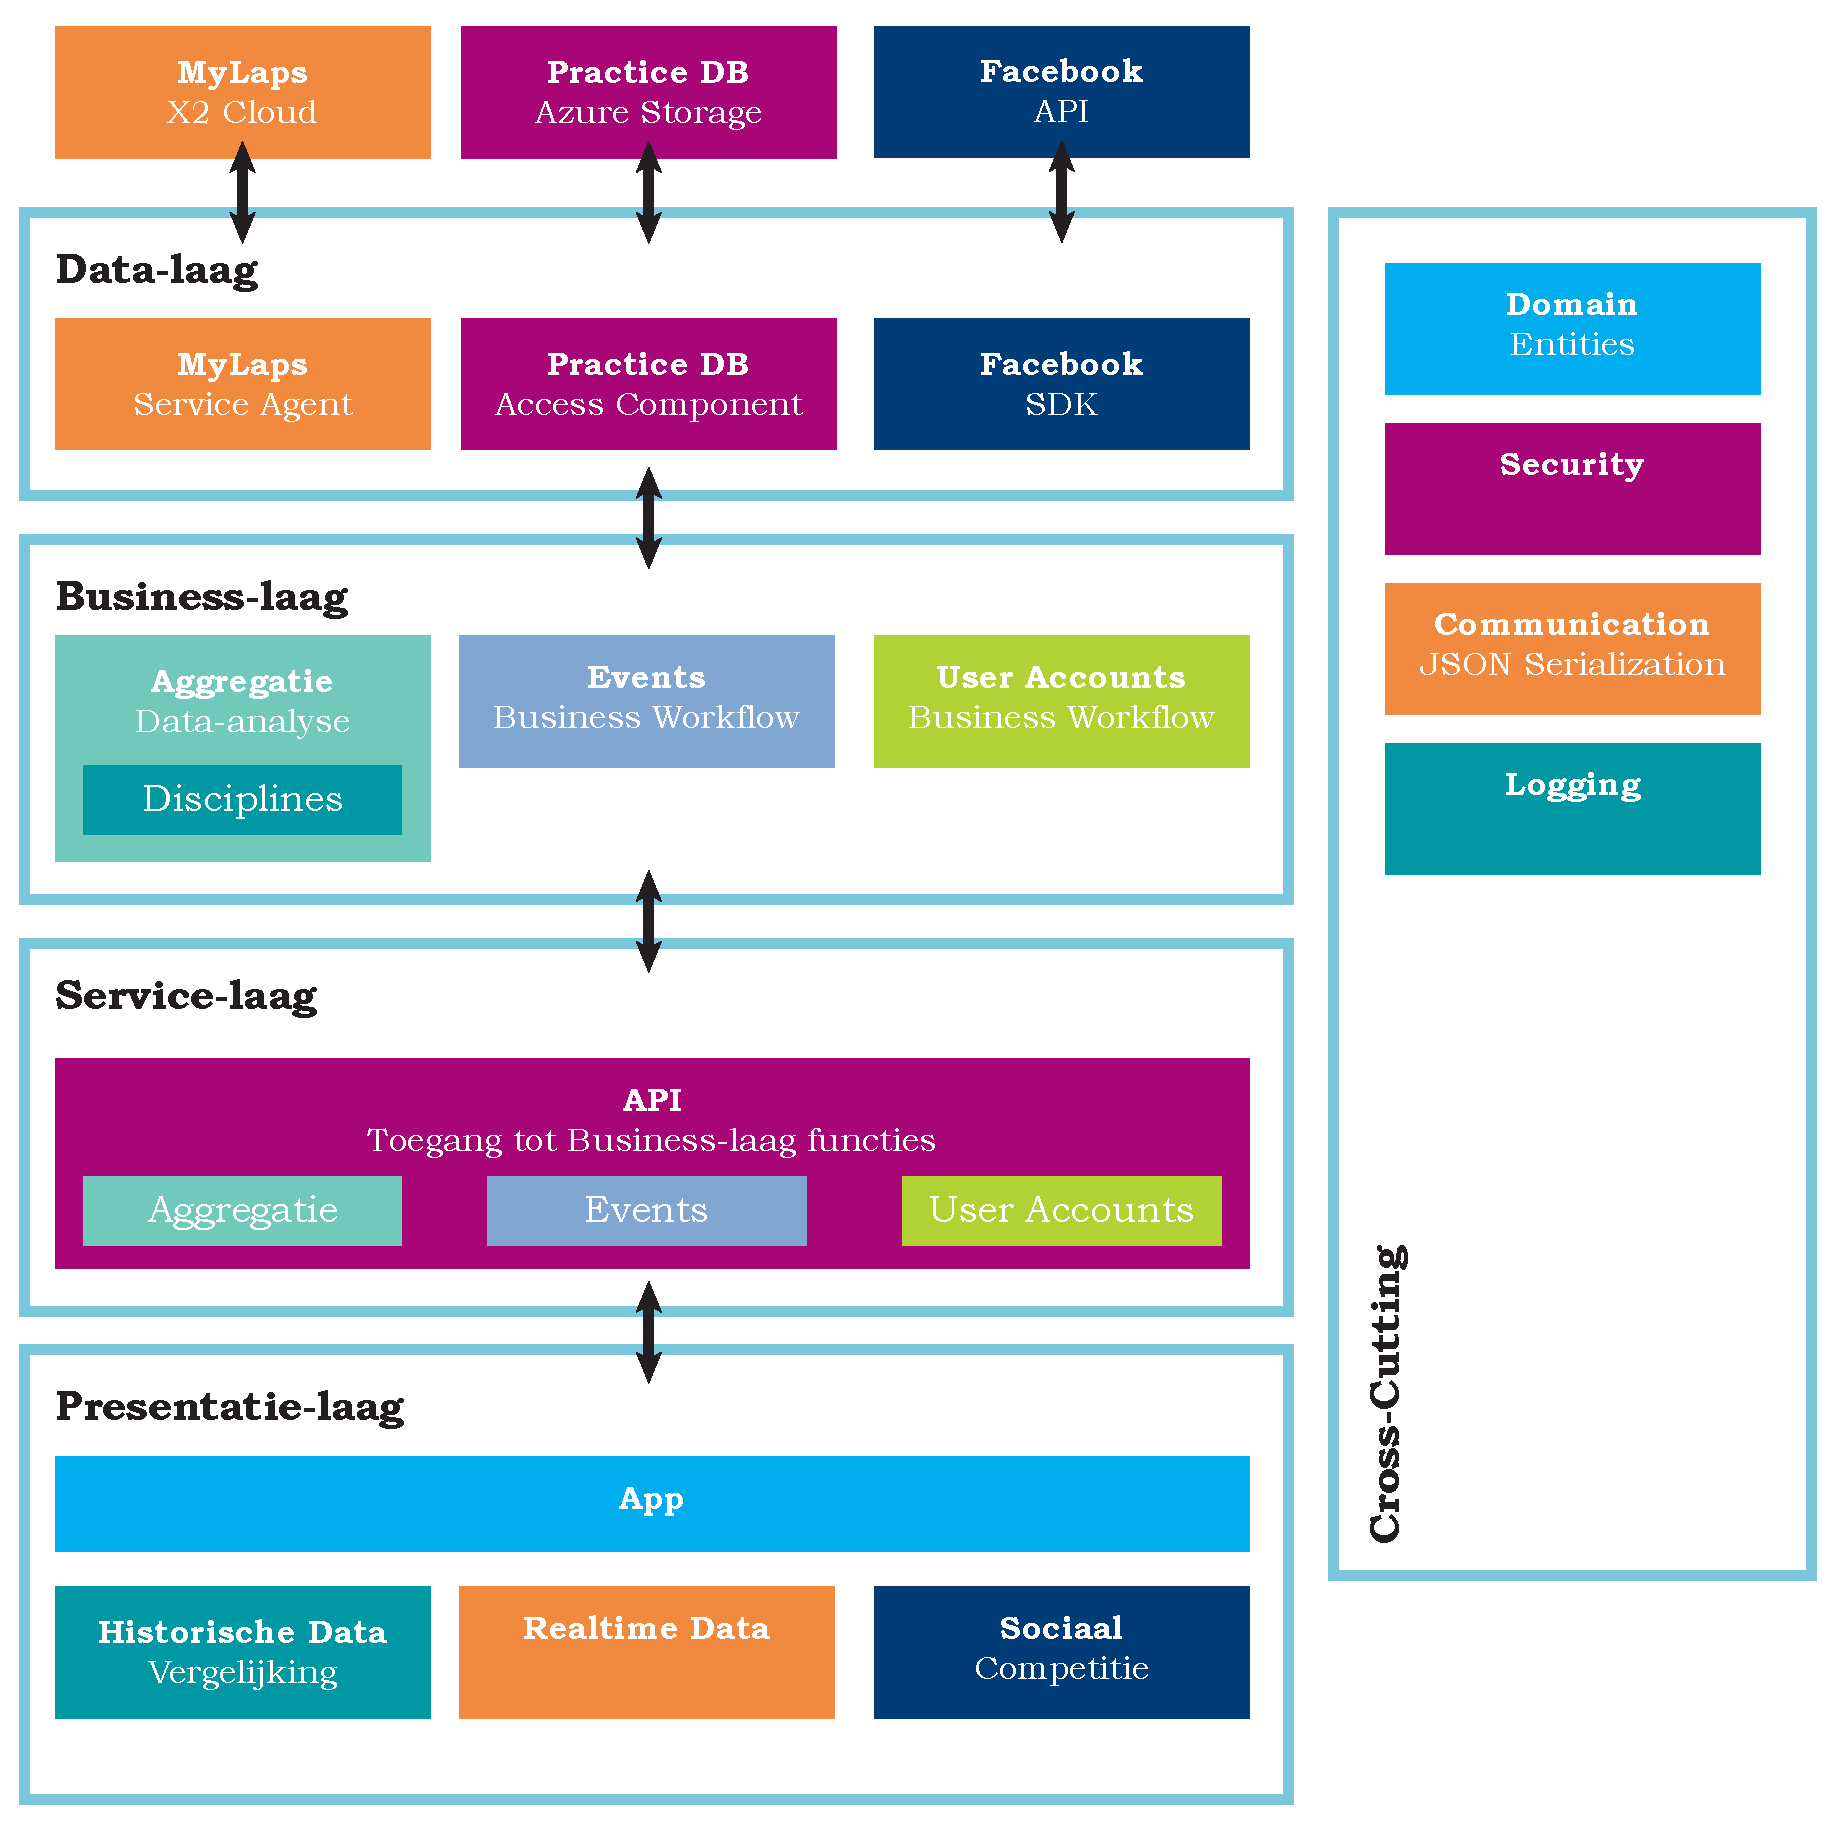
\includegraphics[width=\textwidth]{style/images/Systeem+Architectuur}
\caption{Systeem architectuur}
\label{fig:architecture}
\end{figure}

De data-laag bevat componenten die verbinding kunnen maken met de databases en 
andere services zoals MyLaps Cloud en de Facebook API. De data-laag zet ruwe data 
uit de database om in domein entiteiten en levert deze af bij de business-laag.

De business-laag bevat alle workflows die op de server uitgevoerd moeten worden. 
De workflows zijn in drie categorieen op te delen. Als eerste de Aggregatie
componenten die diverse aggregaties kunnen uitvoeren op data uit de Practice
Database. Ten tweede is er de Event Workflow die bepaald wat er moet gebeuren als
er een event binnenkomt zoals bijvoorbeeld een doorkomst vanaf MyLaps. In het
geval van een doorkomst moet deze bijvoorbeeld worden opgeslagen in de Practice
Database en moeten de aggregaties een iteratie doorlopen. Als derde is er het User
Account component dat acties voor gebruikersacccounts mogelijk maakt. Zo is dit
component belast met het opslaan van nieuwe users, het inloggen met wachtwoord of
met FaceBook, het beheren van groepen en het ophalen van vriendenlijsten.

De service-laag bevat de API. De diverse aanroepen die de clients nodig hebben
worden in de service-laag gekoppeld aan de goede workflow uit de business-laag. De
service-laag zorgt ook voor Caching, waar dat nodig is.

De presentatie-laag bevind zich in de mobiele apps, zij tonen de informatie uit de
service-laag. De presentatie-laag bevat bijvoorbeeld User Interface componenten, 
weergaves voor diverse data types en menu's. Naast de weergave zit er in de apps 
ook een stuk service-laag om te kunnen communiceren met de service-laag op de 
server.